\section{System Architecture}
\label{sec:architecture}

The architecture separates expensive language-model reasoning from cheap
on-device classification. A large language model synthesises interpretable
threshold rules once, offline, from a representative slice of training
traffic. The resulting rule set is a JSON policy that a stateless evaluator
applies to live flows at line rate. Fig.~\ref{fig:architecture} shows the two
phases and the artefact that connects them. This split is what makes the
design deployable on resource-constrained IoT gateways, since the only
runtime dependency is a few dozen threshold comparisons per flow.

\begin{figure}[t]
  \centering
  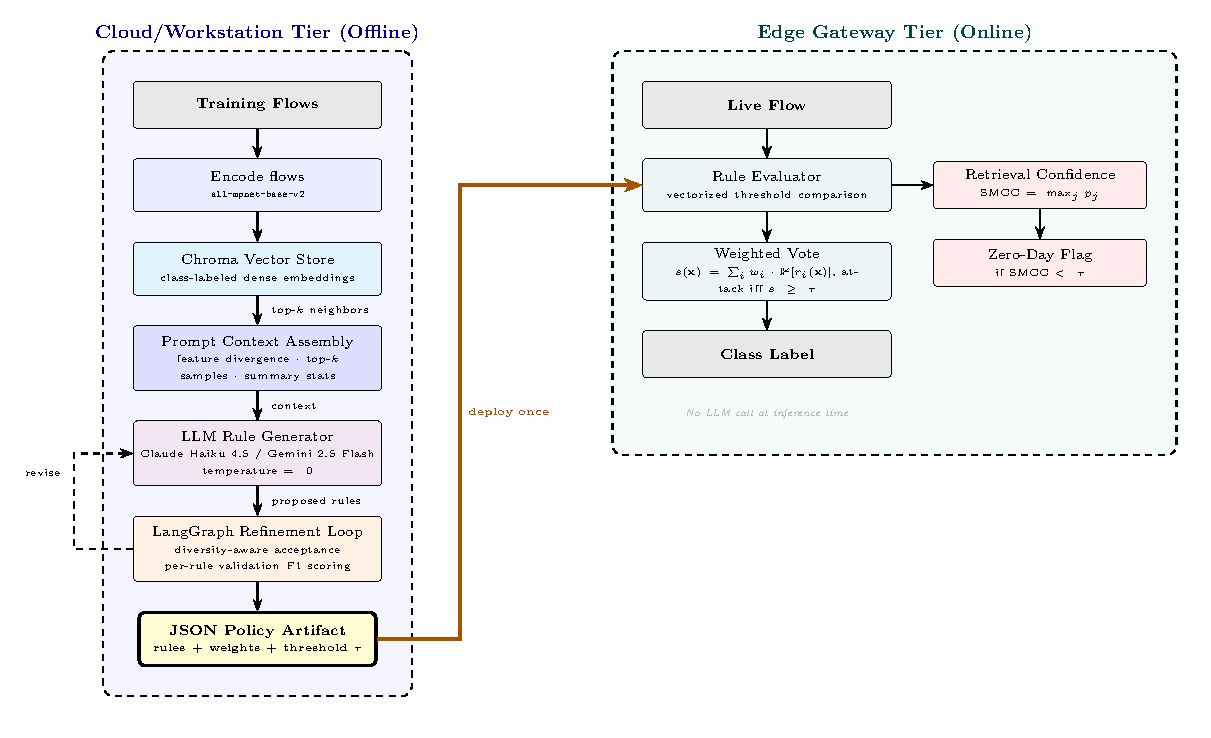
\includegraphics[width=\columnwidth]{figures/fig_architecture.pdf}
  \caption{End-to-end architecture. Offline (left) the system embeds training
    flows into a Chroma vector store, retrieves class-representative neighbours
    by mean-embedding cosine similarity, and prompts Claude Haiku 4.5 to emit
    JSON threshold rules. A LangGraph refinement loop iterates on per-rule
    training F1. Online (right) the deployed rule evaluator scores each flow
    with a vectorised threshold comparison and a majority vote. No
    language-model call is required at inference time.}
  \label{fig:architecture}
\end{figure}

\subsection{Offline Policy Synthesis}
\label{subsec:offline}

Training flows are first featurised into the numeric schema of the source
dataset. Each row is then embedded with
\texttt{sentence-transformers/all-mpnet-base-v2} and persisted in a Chroma
vector store under its class label. For each known class the system computes
a mean embedding and retrieves the top-$k$ nearest neighbours by cosine
similarity. These neighbours act as a compact, class-representative sample
that fits inside the language-model context window without exposing the full
training corpus. Permutation importance ranks the input features and the
highest-ranked names are passed to the prompt alongside the representative
samples. \texttt{claude-haiku-4-5-20251001} (Claude Haiku 4.5) is then
queried at temperature zero and emits one rule set per class as JSON tuples
of the form \texttt{(feature\_name, op, value, target\_class)}, ready for
deployment as ACL-style firewall entries.

A LangGraph state machine closes the loop. Each round evaluates the proposed
rules on the training split, returns per-rule macro-F1 to the model as tool
output, and instructs the model to keep high-scoring rules and revise the
rest. The best-scoring rule set across rounds is retained as the final
policy. The loop terminates after a fixed number of rounds or when the
training-set objective stops improving.

\subsection{Online Detection}
\label{subsec:online}

The deployed component is a stateless rule evaluator. It receives a
featurised flow, evaluates each threshold rule as a vectorised comparison
against the named feature, and emits the majority class label. No model
weights, embeddings, or language-model calls are involved at inference time.
The policy itself is a small JSON file that maps directly onto ACL-style
firewall entries, which keeps the evaluator portable across IoT gateway
hardware. The same evaluator also exposes the retrieved-neighbour confidence
score as an out-of-distribution signal, which Section~\ref{subsec:zeroday}
formalises for zero-day detection.

Section~\ref{sec:framework} formalises the protocols that exercise this
architecture across the four evaluation axes of the paper.
